\chapter{Introduction to Parallel Programming}

\textbf{Resorcess}
\begin{itemize}
    \item \url{https://scrumguides.org/}
    \item \url{http://www.agilemodeling.com/artifacts/userStory.htm}
    \item \url{https://www.uml-diagrams.org/}
\end{itemize}


\section{Intro}
\textit{Sequence} is the instructions that execute \textit{sequencialy}.

\textit{Concurrent}: independend tasks. \textit{Parrallel}: execution at the same time

\textit{speedup}: $S=\frac{T_{old}}{T_{new}}$

Amdahl’s Law
\begin{equation}
  \text{Speedup} = S(n) = \frac{1}{1-p+\frac{p}{n}}.
\end{equation}
where $p$ is the parallel fraction and $1-p$ is the sequential fraction.
%\begin{equation}
%  T(n) = T(1)\left( P + \frac{1}{n}(1-P) \right).
%\end{equation}
%Consiquintly the speedup is
%\begin{equation}
%  S(n) = \frac{T(1)}{T(n)} = \frac{1}{P+\frac{1}{n}(1-P)}.
%\end{equation}

\begin{figure}[!ht]
    \centering
    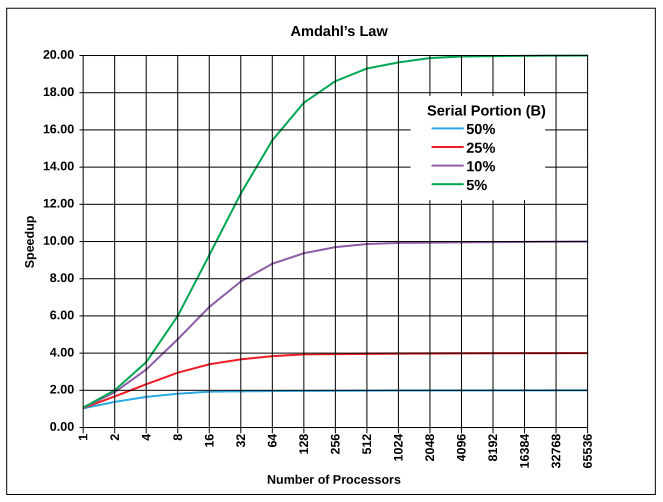
\includegraphics[width=10cm]{\imagesPath/amdahls_law.png}
    \caption{Amdahl’s Law. From~\cite{}}
    % 01 33
\end{figure}



\begin{figure}[!ht]
    \centering
    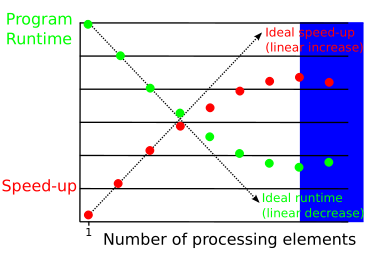
\includegraphics[width=10cm]{\imagesPath/parallel_slowdown.png}
    \caption{Parallel Slowdown. From~\cite{}}
    % 01 34
\end{figure}


\newpage
\subsection{Why parallel computing?}
\begin{itemize}
\item Smaller transistors = faster processors
\item faster processros = increase power consumption
\item increase power consumption = increase heat
\item increase heat = unrealible processors
\end{itemize}
This is why the focus has been on more cores and making programm parallelist will then utilese the resorses of the phisical processor better.

Parallelization of a serial program can eather be done with manually rewriting the program so that more parts become parallel. It can also be done with a translation programs but this is very difficult to do such programs and it has a limited sucess rate.

If we were to have a addor for a sequens of numbers. A parralel approch would be to split the seqens up to diffrent parts and then let the \textbf{master} core add the results. Or let the cours be pared with eatchother and add there results together themselfs.

We devide the the work like a teacher does with exams with the TA's. But this require coordination.
\begin{itemize}
  \item \textit{Communication} between the cores
  \item \textit{Load balance} to split the work evenly
  \item \textit{Synchronization} make sure that one does not get to far ahead of the rest.
\end{itemize}

There are diffrent types of parallel systems those with
\begin{itemize}
  \item \textit{Shared-memmory}, this require coordinate the cores for examening and updating shared memory locations.
  \item \textit{Distributed-memmory}, this require communication to send data between cores. Network?
\end{itemize}

\begin{figure}[!ht]
    \centering
    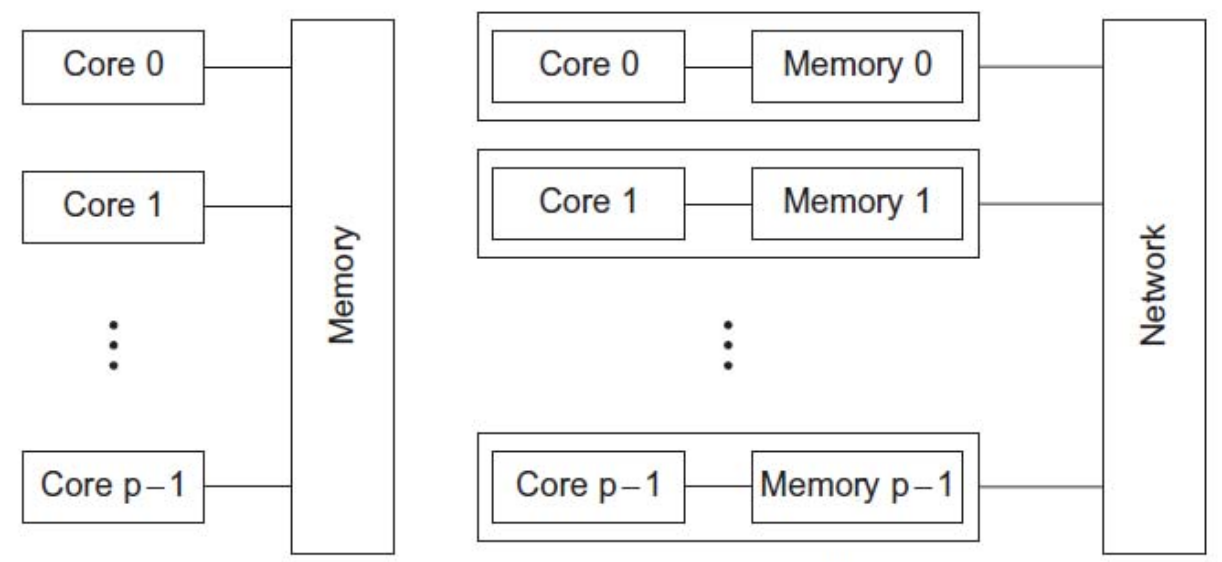
\includegraphics[width=10cm]{\imagesPath/types_of_parallel_systems.png}
    \caption{Types of parallel systems. From~\cite{}}
    % 02.1 31
\end{figure}

\subsection{Basic Concepts}
\subsubsection{Concurrent programing using shared memory}
Good to know
\begin{itemize}
\item Most current multi-processor architectures used shared memory arhitectures.
\item printf is thread-safe.
\item \textit{Deterministic} algorithm means that it will produce the same output every time. Like in a sequential algorithms, unless it depends on externam states.
\item Concurrent programs are ofthen \textit{non-deterministic}, since the output depends on scheduling desissions (\textit{timing-sensitive}).
\item \textit{Race condition} is when the result depend on the timing of its execution.
\item Shared memory doesnt scale well CPU-to-memory is a bottleneck.
\end{itemize}
  

\begin{exampleblock}{\textit{Race condition}}
  What might go wrong when two concurrent calls of count()?

\begin{verbatim}
int x = 0;

int y = x+1;
printf("%d", z);
% ||| concurrent task denotation
int z = x+1;
printf("%d", y);

\end{verbatim}
\end{exampleblock}


\begin{exampleblock}{\textit{Check-Then-Act} error pattern}

\begin{verbatim}
if (check(x)) { act(x); }
\end{verbatim}
  If x changes after it has been change by another process or thread then
  it will still act but it is unwanted behaviur since the if statment is no
  longer true. This can be fixed by using a lock.
\end{exampleblock}

  
\begin{exampleblock}{\textit{Read-Modify-Write} error pattern}
  What might go wrong when two concurrent calls of count()?
\begin{verbatim}
int counter = 0;
count() {
   counter++;
}
\end{verbatim}
  count++ is not a atomic operation, thus it is posible that after counter is read
  it is concurrently modified and therefore will increase by one instead of two.
\end{exampleblock}

This is preventing with \textit{synchronization} to ensure \textit{mutal exclusion} meaning that
no two tasks execute parts of their \textit{critical sections} at the same time.

\begin{definitionblock}{\textit{Dekker's algorithm}}

\begin{BVerbatim}[baseline=c]
// P_0:
flag_0 = true;
while (flag_1) {
  if (turn != 0) {
    flag_0 = false;
    while (turn != 0) {
      // busy wait
    }
    flag_0 = true;
  }
}
// critical section
...
turn = 1;
flag_0 = false;
\end{BVerbatim}
%\quad$\parallel$\quad
\begin{BVerbatim}[baseline=c]
// P_1:
flag_1 = true;
while (flag_0) {
  if (turn != 1) {
    flag_1 = false;
    while (turn != 1) {
      // busy wait
    }
    flag_1 = true;
  }
}
// critical section
...
turn = 0;
flag_1 = false;
\end{BVerbatim}

\end{definitionblock}
There are some limitations: 
\begin{itemize}
  \item only two process
  \item busy waiting is not efficent when comparing to suspending processes
  \item ?assumes that the concurrent execution of P0 and P1 is equivalent to
some interleaving of their instructions (which is often not the case on
modern hardware).
\end{itemize}

Locks can however cause problems for instance \textit{deadloks} where two (or more) tasks are waiting for each other.
\begin{exampleblock}{Deadlock example}
  Consider the following algorithm for copying a file:
  \begin{enumerate}
   \item Open the source file for exclusive access. (Assume that this blocks until
     no other process has the file open. Once this call returns, other processes
     that attempt to open the file block until the file has been closed again by
     the current process.)
   \item Open the destination file for exclusive access.
   \item Copy data from source to destination.
   \item Close the destination file.
   \item Close the source file.
  \end{enumerate}
What can possibly go wrong?
Consider concurrent calls copy("A", "B") and copy("B", "A").
    %0.2.2 19
\end{exampleblock}

Another problem that can occure is \textit{livelocks} where two (or more) tasks are waiting for each
other, like deadlock, but the tasks keep changing theri state, without making progress.
\begin{exampleblock}{Livelocks example}
  Real-life example: two people meet in a narrow corridor. Each tries to be
polite by moving aside to let the other person pass.
    %0.2.2 20
\end{exampleblock}

Problem like \textit{Resource starvation} can also accure, when a task is wating for a resource that keeps getting given to other tasks
\begin{exampleblock}{Starvation example}
  For instance, a (bad) scheduling algorithm might never schedule a task as
  long as there is another task with higher priority.
  % 0.2.2 21
\end{exampleblock}

Althoug the resource will evently be granted to the task (\textit{fairness}). The waiting time is unknown.

\textit{Data race} is when two or more tasks try to access the same shared memory location. This
might even result in the program crashingn.


\subsubsection{Efficency}
Doesent scales well means that the speedup converges. We talk then about \textit{efficency}:
\begin{equation}
  E(n,p) = \frac{S(n,p)}{p}
\end{equation}
If the effeicency decreases as the number of threads increases we call that \textit{weekly scalable}.
%8 functions you need to know for MPI


\subsubsection{Concurrent programing using Distributed memory}
\begin{itemize}
\item Each porcessor has its own private menomy.
\item For communication to accure messegaes has to be sent.
\item Advantages:
  \begin{itemize}
  \item No data race
  \item scales better since it can use any number of processors.
  \end{itemize}
\item Disadvantages:
  \begin{itemize}
  \item High latency to access for data from other process
  \item Expencive to create memory for each 
  \item no uniform address space
  \end{itemize}
\item Memory access
  \begin{itemize}
  \item Uniform memory access (UMA) Shared memory. All access the same way independent on the processor.
  \item symmetric multi-processor (SMP) Shared memory. Treats all processors equaly.
  \item Non-uniform memory access (NUMA) Shared memory. Depends on the memory location.
  \end{itemize}
\item Message passing (send/receive)
  \begin{itemize}
  \item Synchronous: sender is blocked untill receiver calls receive.
  \item Asynchronous: The message is bufferd unteill the receiver calls receive.
  \item Direct Communication: Send message dirictly to a spesified process
  \item Channels: send message via a channel
  \end{itemize}
\end{itemize}

\textbf{moore's law}
%asynchrony
%- cach misses
%- page faults
%- scheaduling quantum use up

\subsubsection{Load balance}
If we split the tasks in the most even way if we dont know how mutch time
it will take then we can use a counter that make everyone take a small task.
Like a tiket counter like in Kjell och kompani.

\subsubsection{Mutal exclusion}
\begin{itemize}
 \item Safety Properties: nothing bad ever happens, e.g. no one take the same ticket.
 \item Liveness Properties: something good happens eventualy, e.g. eventialy some get a ticket.
Fareness
\end{itemize}

Flag protocal
\begin{itemize}
\item Alice protocal
  \begin{itemize}
    \item Raise flag
    \item Wait until Bob’s flag is down
    \item Unleash pet
    \item Lower flag when pet returns
  \end{itemize}
\item Bob protocal
  \begin{itemize}
    \item Raise flag
    \item While Alice’s flag is up
      \begin{itemize}
        \item Lower flag
        \item Wait for Alice’s flag to go down
        \item Raise flag
      \end{itemize}
    \item Unleash pet
    \item Lower flag when pet returns
  \end{itemize}
\end{itemize}


\section{Threads and locks}
\subsection{PThreads}
Posix Thread API is the standard thread API. A instead of a function.
Threads are a more portability and ease of use.

\subsubsection{Stack}
\begin{itemize}
\item Stack: when we call another function and the other function calles. So the latest will return before the once before so the last alocated is removed first.
\item Each tread has to have its own stack becaseu otherwise the stack would be brocken. (lodgical)
\item The stack is allocated at the beginng and it is devided to the threads.
\end{itemize}

\subsubsection{Commands}
\begin{itemize}
\item pthread\_create, starts and create
\item pthread\_join, will just wait everyone else
\item pthread\_exit, will just exit the thread, it is caled from a thread
\end{itemize}
\begin{itemize}
\item pthreads\_mutex\_lock, lock the lock
\item pthreads\_mutex\_unlock, unlock the lock
\item pthreads\_mutex\_init, can use std::mutex but this create and initialaze the lock.
\end{itemize}

\subsection{Locks}
Types of mutexes
\begin{itemize}
\item Normal, if you call the lock again it deadlock. Will just stop if it is called. Less overhead needs no counter or anything.
\item Recursive (re-entrant), allow to call mutex multiple times.
\item Error-check, it give error if called multiple times.
\end{itemize}
\textit{Producer-Consumer} is posible with locks.

\textit{Condition variables} are varibles which can be used to synchronization by
sending mesage/signal to the verible. If not try get a message and signals when it is not locked.
this is done with pthreads\_con\_wait. also signal, broadcast, init, destroy.
We run \textit{try-lock} first then we do conditional variables if that doesent work.
Most of the time it should be free so it is faster.

\textit{Attributes} can be set to change the default attributes for threads, mutex, conditional varibles.
For instance it is posible to spesifify the size of the stack for that is created for each thread.
And also if mutex should be normal, recursive, or error-check.

\textit{reader-writer locks} is a good option when it ixpected to be many read but few writes.
It can only be one writers but many reader. It will also wake up all readers when we write the locks.

\textit{Barriers} are used to make every one stop until every one is there and then carry on.


% Lecture 5
Must of the curent devices are \textit{MIMD} (Multiprocessors). There are other kinds of achitectures
like SISD (Uniprocessor), and SIMD (Vector). In MIMD we have Memory Contention
(can`t access the same memory at the same time), Communication contention (accessing the bus),
and communication latency (time it takes to communicate memmory or other processor).

\subsection{Spin-lock}
We keep trying until we get it.

\subsubsection{TAS}
Test-And-Set Lock, a atomic operation that set avalue of a bolean. The return is the prior value.

\begin{BVerbatim}[baseline=c]
class TASlock {
  AtomicBoolean state =
    new AtomicBoolean(false);

  void lock() {
    while (state.getAndSet(true)) {}
  }
  
  void unlock() {
    state.set(false);
  }
}
\end{BVerbatim}

\textbf{Remember} \textit{Cache hit} and \textit{Cache miss}.
The cash is not nesessaraly shared between processes thus when data
is accessed from memory it will be stored in the cash of the processor,
when another processor acces the same data it will talk with the bus wich
will say that another process has the data and get it from there cach instead of
the main memory. When modifing the data it will have to say to the other process
that it is obsolite and then when the other process access the data again it will
take the value from the first processors cach.
This is caled \textit{Cache Coherence}.
\textit{Cash coherents problem} if we modify in some chach what should we update to.
\textit{Write-Back Caches}, we need a protocal
to write the data back to memory and to the other processors cach.
Write-Back caches, it is expencive to write it to memory wo we wait until the end? we prospone it
For this protocal a \textit{cach entry} has tree states \textit{Invalid}, \textit{Valid}, \textit{Dirty}.


\subsubsection{TATAS}
We need to write to the lock to read it, two or more can not write to the bus at the same time.
That is why we Test-And-Test-and-Set, check if it is free first. 
It is faster since we avoid memory colisions since only one is writing to the bus at the same time so we will likely write at the same time and then we need to fix it. One can write but many can look at it.

When I want to write to the data i say that to the bus first and therefore everyone else will say theres
data is invalid. Cash is cold when its nothing it it.
TAS Only one has the lock and we continue spinn on it and get a cach miss every time.

\begin{BVerbatim}[baseline=c]
class TATASlock {
  AtomicBoolean state =
    new AtomicBoolean(false);

  void lock() {
    while (true)
       while (state.get()) {}
       if (!state.getAndSet(true))
          return;
  }
}
\end{BVerbatim}


\subsubsection{Exponential backoff lock}
Exponential backoff, if there is a conflict again then we incerease the delay.
%We set random delay we set the first time.

Exponential Backoff lock

\begin{BVerbatim}[baseline=c]
  public class Backoff implements lock {
    public void lock() {
      int delay = MIN_DELAY;
      while (true) {
        while (state.get()) {}
        if (!lock.getAndSet(true))
           return;
        sleep(random() % delay);
        if (delay < MAX_DELAY)
           delay = 2 * delay;
      }
    }}
\end{BVerbatim}

contention problem
if contention is unlikely then TAS is the best since it is less operation

\subsubsection{?}
We give up the process and when we get an indication when it is unlocked.
Sequential bottleneck, we sequentialise the prarallel program.


\subsection{Queue Locks}
When there is contention on the lock it is better to use a queue lock.
Since it prevent threads spining only one lock, instead you spinn on the
the lock that is not already taken.

Somtimes a thread need to abort a lock, but with a queue this is difficult since
it is no wait free, it requires cleaning up and cant immediate return.
Have a queue were thread spin on the first false slot in the queue.

\subsubsection{Anderson queue lock}
A array of false values that when each thread sets the most resent element
to true when it wants to take the lock. This require the number of threads
to be defined in order to create a array of correct size.

\begin{BVerbatim}[baseline=c]
public lock() {
  mySlot = next.getAndIncrement();
  while (!flags[mySlot % n]) {};
  flags[mySlot % n] = false;
}
public unlock() {
  flags[(mySlot+1) % n] = true;
}
\end{BVerbatim}
Memmory needed:
\begin{equation}
  O(L\cdot N)
\end{equation}
where L is the number of locks and N is the number of threads.


\subsubsection{CLH Queue Locks}
The size of the queue is dynamic unlike anderson queue lock.
The queue is represented with a linked list.
Initialy there is only one element int the queue, then when
the a thread takes the lock, it creates a new element, but still
point the the first element. The next thread creates a new
element and point to the element created by the first thread.
The second thread spinns on the element it points to (acctualy a copy).
Then when the first releases the lock the second aquire the lock and
only the element that it created remains.
There is also a tail that points to the next element.

Memmory needed:
\begin{equation}
  O(L+N)
\end{equation}
where L is the number of locks and N is the number of threads.

This does not work on unchached NUMA architecture, i.e. no caches.

\begin{BVerbatim}[baseline=c]
class CLHLock implements Lock {
  AtomicReference<Qnode> tail;
  ThreadLocal<Qnode> myNode
    = new Qnode();

  public void lock() {
    Qnode pred = tail.getAndSet(myNode);
    while (pred.locked) {}
  }
  public void unlock() {
    myNode.locked.set(false);
    myNode = pred;
  }
}
\end{BVerbatim}

\subsubsection{MCS Locks}
Unlike CLH that spinns on predecessor’s memmory, MCS spinns on a local
memory only, which make it faster memmory access. It works imilarly but nowait
there is a linked list that point to a memmory location local the each thread.

\begin{BVerbatim}[baseline=c]
class MCSLock implements Lock {
  AtomicReference tail;
  public void lock() {
    Qnode qnode = new Qnode();
    Qnode pred = tail.getAndSet(qnode);
    if (pred != null) {
      qnode.locked = true;
      pred.next = qnode;
      while (qnode.locked) {}
    }
  }

  public void unlock() {
    if (qnode.next == null) {
      if (tail.CAS(qnode, null)
         return;
      while (qnode.next == null) {}
    }
    qnode.next.locked = false;
  }
}
\end{BVerbatim}


\section{OpenMP}
OpenMP creates and terminate threads automaticly. We give compiling instructions
to spesify where and how this should be done by using directives based on the pragma compiler directives.
We can think of it like pthread under the hod.

\subsection{Loops}
\subsubsection{Loop carried dependencies}
Loops can only be parallelist if there is no \textit{loop carried dependencies}.
\begin{exampleblock}{\textit{Check-Then-Act} error pattern}
Example of modifing loop to remove loop carried dependencies.
\begin{BVerbatim}[baseline=c]
int i,j,A[MAX];
j = 5;
for (i=0;i<MAX;i++){
  j+=2;
  A[i]=big(j);
}
\end{BVerbatim}

This can be modefined to:
\begin{BVerbatim}[baseline=c]
int i,j,A[MAX];
#pragma omp parallel for
for (i=0;i<MAX;i++){
  j = 5 + 2*(i+1);
  A[i]=big(j);
}
\end{BVerbatim}
%https://www.youtube.com/watch?v=iPb6OLhDEmM&list=PLLX-Q6B8xqZ8n8bwjGdzBJ25X2utwnoEG&index=11
\end{exampleblock}

\subsubsection{Scheduling}
\begin{itemize}
  \item staric\: define a strict chunk size which does not change over runtime.
  \item dynamic\: similar to counter when load balancing.
  \item guided\: chunk size is predefined but changes during runtime.
  \item automatic\: let the compiler define how to load balance.
  \item runtime\: scheduling is defined during runtime.
\end{itemize}

\subsubsection{Reduction}
\textit{Reduction} is verrey common.
\begin{BVerbatim}[baseline=c]
double ave = 0.0, A[MAX]; int i;
for (i=0;i<MAX;i++){
  ave += A[i];
}
ave = ave/MAX;
\end{BVerbatim}
This is a form of loop carried dependencie. Since have depends on the previus iterations
since you read and then update it so the final value is a commulation of the iterations in squence.


\begin{BVerbatim}[baseline=c]
  reduction (op: list)
\end{BVerbatim}
Op i the type of operation, e.g. ``+'', and list is the varible that will change.
This will create local instances of the varible and then add them together afterwords.
The initial value is ``0'' for the ``+'' operations of the list. If it is times then it needs to be ``1'' since otherwise it would alwase be 0.

\subsection{Syncronisation}
\subsubsection{Barrier}
openmp put bariers for you, e.g. when there is two loops at a row.
\textit{Nowait}: dont put a barrier here.
For those cases where it is no barrier by default you need to put a \textit{barrier}.
\textit{master} only the master thread does this, there is no syncronisations so we have to but a barrier aterwords if we want the other threads to wait until the master is done.
\textit{single} only the first thread that reatch it will do the task.
Workshare construct like single and master the compiler alwase but a barrier afterwords.
another one is \textit{section} with means that one will do this and others will do the other section.

\subsubsection{Looks}

\subsection{Environment Variables}
\begin{itemize}
  \item OMP\_NUM\_THREADS: set the number of thread to use. No garante.
  \item OMP\_STACKSIZE: limit the stack size to prevent system crash.
  \item OMP\_WAIT\_POLICY ACTIV|PASSIVE: To spin on locks or put thread to sleap.
  \item OMP\_PROC\_BIND TRUE|FALSE: Bind thread to a spesific process for inctance if you want to make sure it access the same chach and not have to access cach fether away in the cach hiracry.
\end{itemize}
  
\subsection{Data Environment}
Private on the stack. Shared on the heap.
\begin{itemize}
  \item SHARED\: Every thread has the same version.
  \item PRIVATE\: Every thread has there local version. Un enitialised.
  \item FIRSTPRIVATE\: Same as privete but initialized to the value given.
  \item LASTPRIVATE\: Save the last value of the variable.
  \item DEFAULT(PRIVATE|SHARED|NONE)\: Set the default.
\end{itemize}

\section{MPI}
Message Passing Interface (MPI) a library specification. Many implementations with subtle
diffrences between implementations. As the name sugest data is chared by sending messages
since processes do not share memory like theads does. MPI allowes distrebution of work accross
multiple machines.

%Data Parallel SIMD
%Task Parallel MIMD

MPI when there is a error from MPI the program will crash.
The MPI suppervices wil crash so all MPI programs runing will crash.

Processes can be collected in a \textit{group}. Messages that are sent contain a \textit{tag},
which sets the \textit{context} of the message in order to achive point-to-point communication.
Groups and context together formes a \textit{communicator}. Each process as a id called \textit{rank} starting from 0. 

There is a number for MPI data types that can be used to send messages.

\begin{BVerbatim}[baseline=c]
  MPI_Init
  // Everyting in between thise two will run with MPI
  MPI_Finalize
\end{BVerbatim}

when we cal the exec program we spesifiy all other process so we can execute for multiple machines.
Int tag the data, so we can determin wheter or not to process it by the reciver.

\subsection{Basic functions}
\begin{BVerbatim}[baseline=c]
  MPI_COMM_SIZE  // number of processes involved in a communicator
  MPI_COMM_RANK  // rank of the calling process in the communicator
  MPI_Send  // blocking send
  MPI_Recv  // blocking recieve
  MPI_BCAST  // bradcast to all other in the communicator
  MPI_REDUCE  // combind all data from all the processes to 
\end{BVerbatim}

\subsection{Deadlock with MPI}
Deadlock may still happen.

\begin{BVerbatim}[baseline=c]
  Send(1) Send(0)
  Recv(1) Recv(0)
\end{BVerbatim}
There is no space for we need to wait untill it is space at the reciver.

Rreliing on the buffer to execute properly is unsafe since ther migth be deadlock, if not implemented
correctly. If we want to debug we can run MPI\_Ssend instead. The extra ``s'' stands for synchronous
which garrently that it will block untill it is recived.

%If you want to test your program do a non-blocking send/recv
Non-blocking send/recv

\begin{BVerbatim}[baseline=c]
  Isend(1) Irecv(0)
  Irecv(1) Isend(0) 
  Waitall  Waitall
\end{BVerbatim}
%https://www.mcs.anl.gov/research/projects/mpi/tutorials/perf/

\subsection{Brodcast and reduce}
\textit{tree-structure communication}.
\textit{Reduce} Need to spesify a interval of ..
\textit{Allreduce} all processes do the reduction and get the value.

When using reduce you spesify the number a value operator like MPI\_SUM or MPI\_LOR that does operation
to all the results in a group.

MPI comes with suport with messure preformance/time MPI\_Wtime. There is also barriers (MPI\_Barrier). We should have a barrier before we messure time so one process does not finnish before tthe other and mesur the time.

\subsection{Other functions}
\begin{BVerbatim}[baseline=c]
  MPI_Comm_split  // Create new communicator
  MPI_Scatter  // Similar to broadcast but send chunks of the data not the same
  MPI_Gather  // Similar to reduce but process 0 does all the work
  MPI_Sendrecv  // Both send and recv 
\end{BVerbatim}